\documentclass{beamer} % blue; brown; gray; red;
\usepackage{beamerthemesplit}
\usepackage{beamerthemeshadow}
\usepackage{animate}
\usepackage{movie15}
%\usepackage[numbered]{mcode}
\usepackage{graphics}
\usepackage{colortbl}
\usepackage{pgf,pgfarrows,pgfnodes,pgfautomata,pgfheaps}
\usepackage{amsmath,amssymb}

%%%%%%%%%%%%%%%%%%%%%%%%%%%%%%%%%%%%%%%%%%%%%%%%%%%%%%
\usepackage{xeCJK}
\usepackage{fontspec}
\setCJKmainfont[BoldFont=simhei.ttf]{simkai.ttf}
%\setCJKsansfont{simhei.ttf}
%\setCJKmonofont{simfang.ttf}
%%%%%%%%%%%%%%%%%%%%%%%%%%%%%%%%%%%%%%%%%%%%%%%%%%%%%%

\usetheme{Warsaw}
%别的主题:Bergen,Boadilla,Madrid,AnnArbor,CambridgeUS,Pittsburgh, Rochester.
%有导航栏:Antibes,JuanLesPins,Montpellier,
%有内容的:Berkeley,PaloAlto,% Goettingen,Marburg,Hannover
%小导航栏:Berlin,Ilmenau,Dresden,Darmstadt, Frankfurt,Singapore,Szeged,
%章节表单:Copenhagen,Luebeck,Malmoe,Warsaw
\beamertemplateshadingbackground{red!10}{structure!10}
\beamertemplatesolidbackgroundcolor{white!90!blue}
\beamertemplatetransparentcovereddynamic
\beamertemplateballitem
\beamertemplatenumberedballsectiontoc
%\beamertemplatelargetitlepage
\beamertemplateboldpartpage

\usecolortheme{sidebartab}
%beetle,crane,dove,fly,seagull,wolverine,beaver
\renewcommand{\raggedright}{\leftskip=0pt \rightskip=0pt plus 0cm}
\raggedright
%%%%%%%%%%%%%%%%%%%%%%%%%%%%%%%%%%%%%%%%%%%%%%%%%%%%%%%%%%%%%%%%%%%%%%%%%%
\graphicspath{{figures/}}
%%%%%%%%%%%%%%%%%%%%%%%%%%%%%%%%%%%%%%%%%%%%%%%%%%%%%%%%%%%%%%%%%%%%%%%%%%
\makeatletter
\usefoottemplate{ %重新定义页脚,加入作者,单位,单位图标,和文档标题
  \vbox{\tiny%
    \hbox{%
      \setbox\beamer@linebox=\hbox to\paperwidth{%
        \hbox to.5\paperwidth{
            \hfill\tiny\color{white}
                  \textbf{\insertshortauthor\quad\insertshortinstitute}
            \hskip .1cm\lower 0.2em\hbox{
\includegraphics[height=0.25cm]{./figures/CAS.pdf}}
            \hskip.3cm}%
        \hbox to.5\paperwidth{
            \hskip.3cm\tiny\color{white}
                  \textbf{\insertshorttitle}\hfill}\hfill}%
      \ht\beamer@linebox=2.625ex%
      \dp\beamer@linebox=0pt%
      \setbox\beamer@linebox=\vbox{\box\beamer@linebox\vskip1.125ex}%
      \color{structure}\hskip-\Gm@lmargin\vrule width.5\paperwidth
      height\ht\beamer@linebox\color{structure!70}\vrule width.5\paperwidth
      height\ht\beamer@linebox\hskip-\paperwidth%
      \hbox{\box\beamer@linebox\hfill}\hfill\hskip-\Gm@rmargin}
  }
}
\makeatother
%%%%%%%%%%%%%%%%%%%%%%%%%%%%%%%%%%%%%%%%%%%%%%%%%%%%%%%%%%%%%%%%%%%%%%%%%%


\begin{document}
\title{细胞吸入微管道的耗散粒子动力学(DPD)模拟}
\subtitle{2012颗粒材料计算力学会议~~张家界}
\institute[中国科学院力学研究所]{中国科学院力学研究所}
\author{周吕文 \and 刘谋斌}
\date{2012年09月21日}

\pgfdeclaremask{zhou}{./Logo/CAS.pdf}
\pgfdeclareimage[mask=zhou,height=2.5cm]{zhou}{./figures/CAS.pdf}
\titlegraphic{\pgfuseimage{zhou}}
%%%%%%%%%%%%%%%%%%%%%%%%%%%%%%%%%%%%%%%%%%%%%%%%%%%%%%%%%%%%%%%%%%%%%%%%%%
\frame[plain]{\titlepage} % 产生主题页,plain选项表示不显示页眉页脚等内容
\titlegraphic{\pgfuseimage{title}}
\AtBeginSection[]{ % 在每个Section前都会加入的Frame
  \frame<handout:0>{
    \frametitle{提纲}
    \tableofcontents[current,currentsubsection]
  }
}
\frame[Outline]{\frametitle{提纲}\tableofcontents}
%%%%%%%%%%%%%%%%%%%%%%%%%%%%%%%%%%%%%%%%%%%%%%%%%%%%%%%%%%%%%%%%%%%%%%%%%%

\section{耗散粒子动力学}
%%%%%%%%%%%%%%%%%%%%%%%%%%%%%%%%%%%%%%%%%%%%%%%%%%%%%%%%%%%%%%%%%%%%%%%%%%
\subsection{简介}
\frame{ \frametitle{耗散粒子动力学简介}
  \begin{itemize}
  \item 耗散粒子动力学(DPD)是一种适合模拟简单和复杂流体动力学和流变性能的介观
        尺度方法.
  \item 由Hoogerbrugge与Koelman首先提出, 旨在解决经典分子动力学难以解决的流体
        时间和空间尺度问题.
  \item 应用: 各类复杂的流体流动, 如相分离, 蛋白质等大分子悬浮, 表面活性剂, 胶
        体输运, 稀释聚合物溶液, 生物薄膜, 以及介观尺度的多相流动现象.
  \end{itemize}
}
%%%%%%%%%%%%%%%%%%%%%%%%%%%%%%%%%%%%%%%%%%%%%%%%%%%%%%%%%%%%%%%%%%%%%%%%%%
\subsection{基本思想}
\frame{\frametitle{运动方程}
\begin{itemize}
\item 牛顿运动方程描述DPD粒子运动
  \[
  \frac{d\mathbf{r}_i}{dt} = \mathbf{v}_i,   
  \frac{d\mathbf{v}_i}{dt} = \mathbf{f}_i = \mathbf{f}_i^{\text{int}} + \mathbf{f}_i^{\text{ext}}
  \]
 
\item DPD粒子间作用力包括保守力, 耗散力及随机力:
  \[
  \mathbf{F}_{ij}^C = a_{ij}w^C(r_{ij})\mathbf{\hat{r}}_{ij}
  \]
  \[
  \mathbf{F}_{ij}^D = -\gamma w^D(r_{ij})\Big(\mathbf{\hat{r}}_{ij}\cdot \mathbf{v}_{ij}\Big)\mathbf{\hat{r}}_{ij}
  \]
  \[
  \mathbf{F}_{ij}^R = \sigma w^R(r_{ij})\xi_{ij}\mathbf{\hat{r}}_{ij}
  \]
保守力权函数$w^C(r_{ij})$, 一般取为$1-r_{ij}$.
\end{itemize}
}
%%%%%%%%%%%%%%%%%%%%%%%%%%%%%%%%%%%%%%%%%%%%%%%%%%%%%%%%%%%%%%%%%%%%%%%%%%

\frame{\frametitle{热力学平衡条件}
\begin{itemize}
\item 为了维持系统温度不变, 根据随机耗散理论及能量守恒定律, 耗散力与
随机力系数, 以及耗散力权函数和随机力权函数必须满足以下关系

\[
\sigma^2=2\gamma k_BT
\]
\[
w^D(r_{ij})=\Big[w^R(r_{ij})\Big]^2
\]

耗散力权函数$w^D(r_{ij})$一般取$(1-r_{ij})^2$
\end{itemize}
}

%%%%%%%%%%%%%%%%%%%%%%%%%%%%%%%%%%%%%%%%%%%%%%%%%%%%%%%%%%%%%%%%%%%%%%%%%%
\subsection{简单的算例}
\frame{\frametitle{简单流体的模拟}
\begin{center}
  \animategraphics[width=0.9\textwidth, autoplay, loop]{5}{./animate/Poise/}{1}{20}
\end{center}
}

\frame{\frametitle{高分子链在微直通道中的运动}
\begin{center}
\animategraphics[width=0.9\textwidth, autoplay, loop]{5}{./animate/Chain=/}{1}{30}
\end{center}
}
\frame{\frametitle{高分子链在微缩通道中的运动}
\begin{center}
  \animategraphics[width=0.9\textwidth, autoplay, loop]{5}{./animate/ChainT/}{1}{30}
\end{center}
}

\frame{\frametitle{高分子链在微缩通道中的运动}
\begin{center}
  \animategraphics[width=0.9\textwidth, autoplay, loop]{5}{./animate/ChainY/}{1}{30}
\end{center}
}

\section{细胞力学模型}
\subsection{细胞吸入实验简介}
\frame{\frametitle{细胞吸入实验简介}
  \begin{columns}
  \begin{column}[b]{0.52\textwidth}
 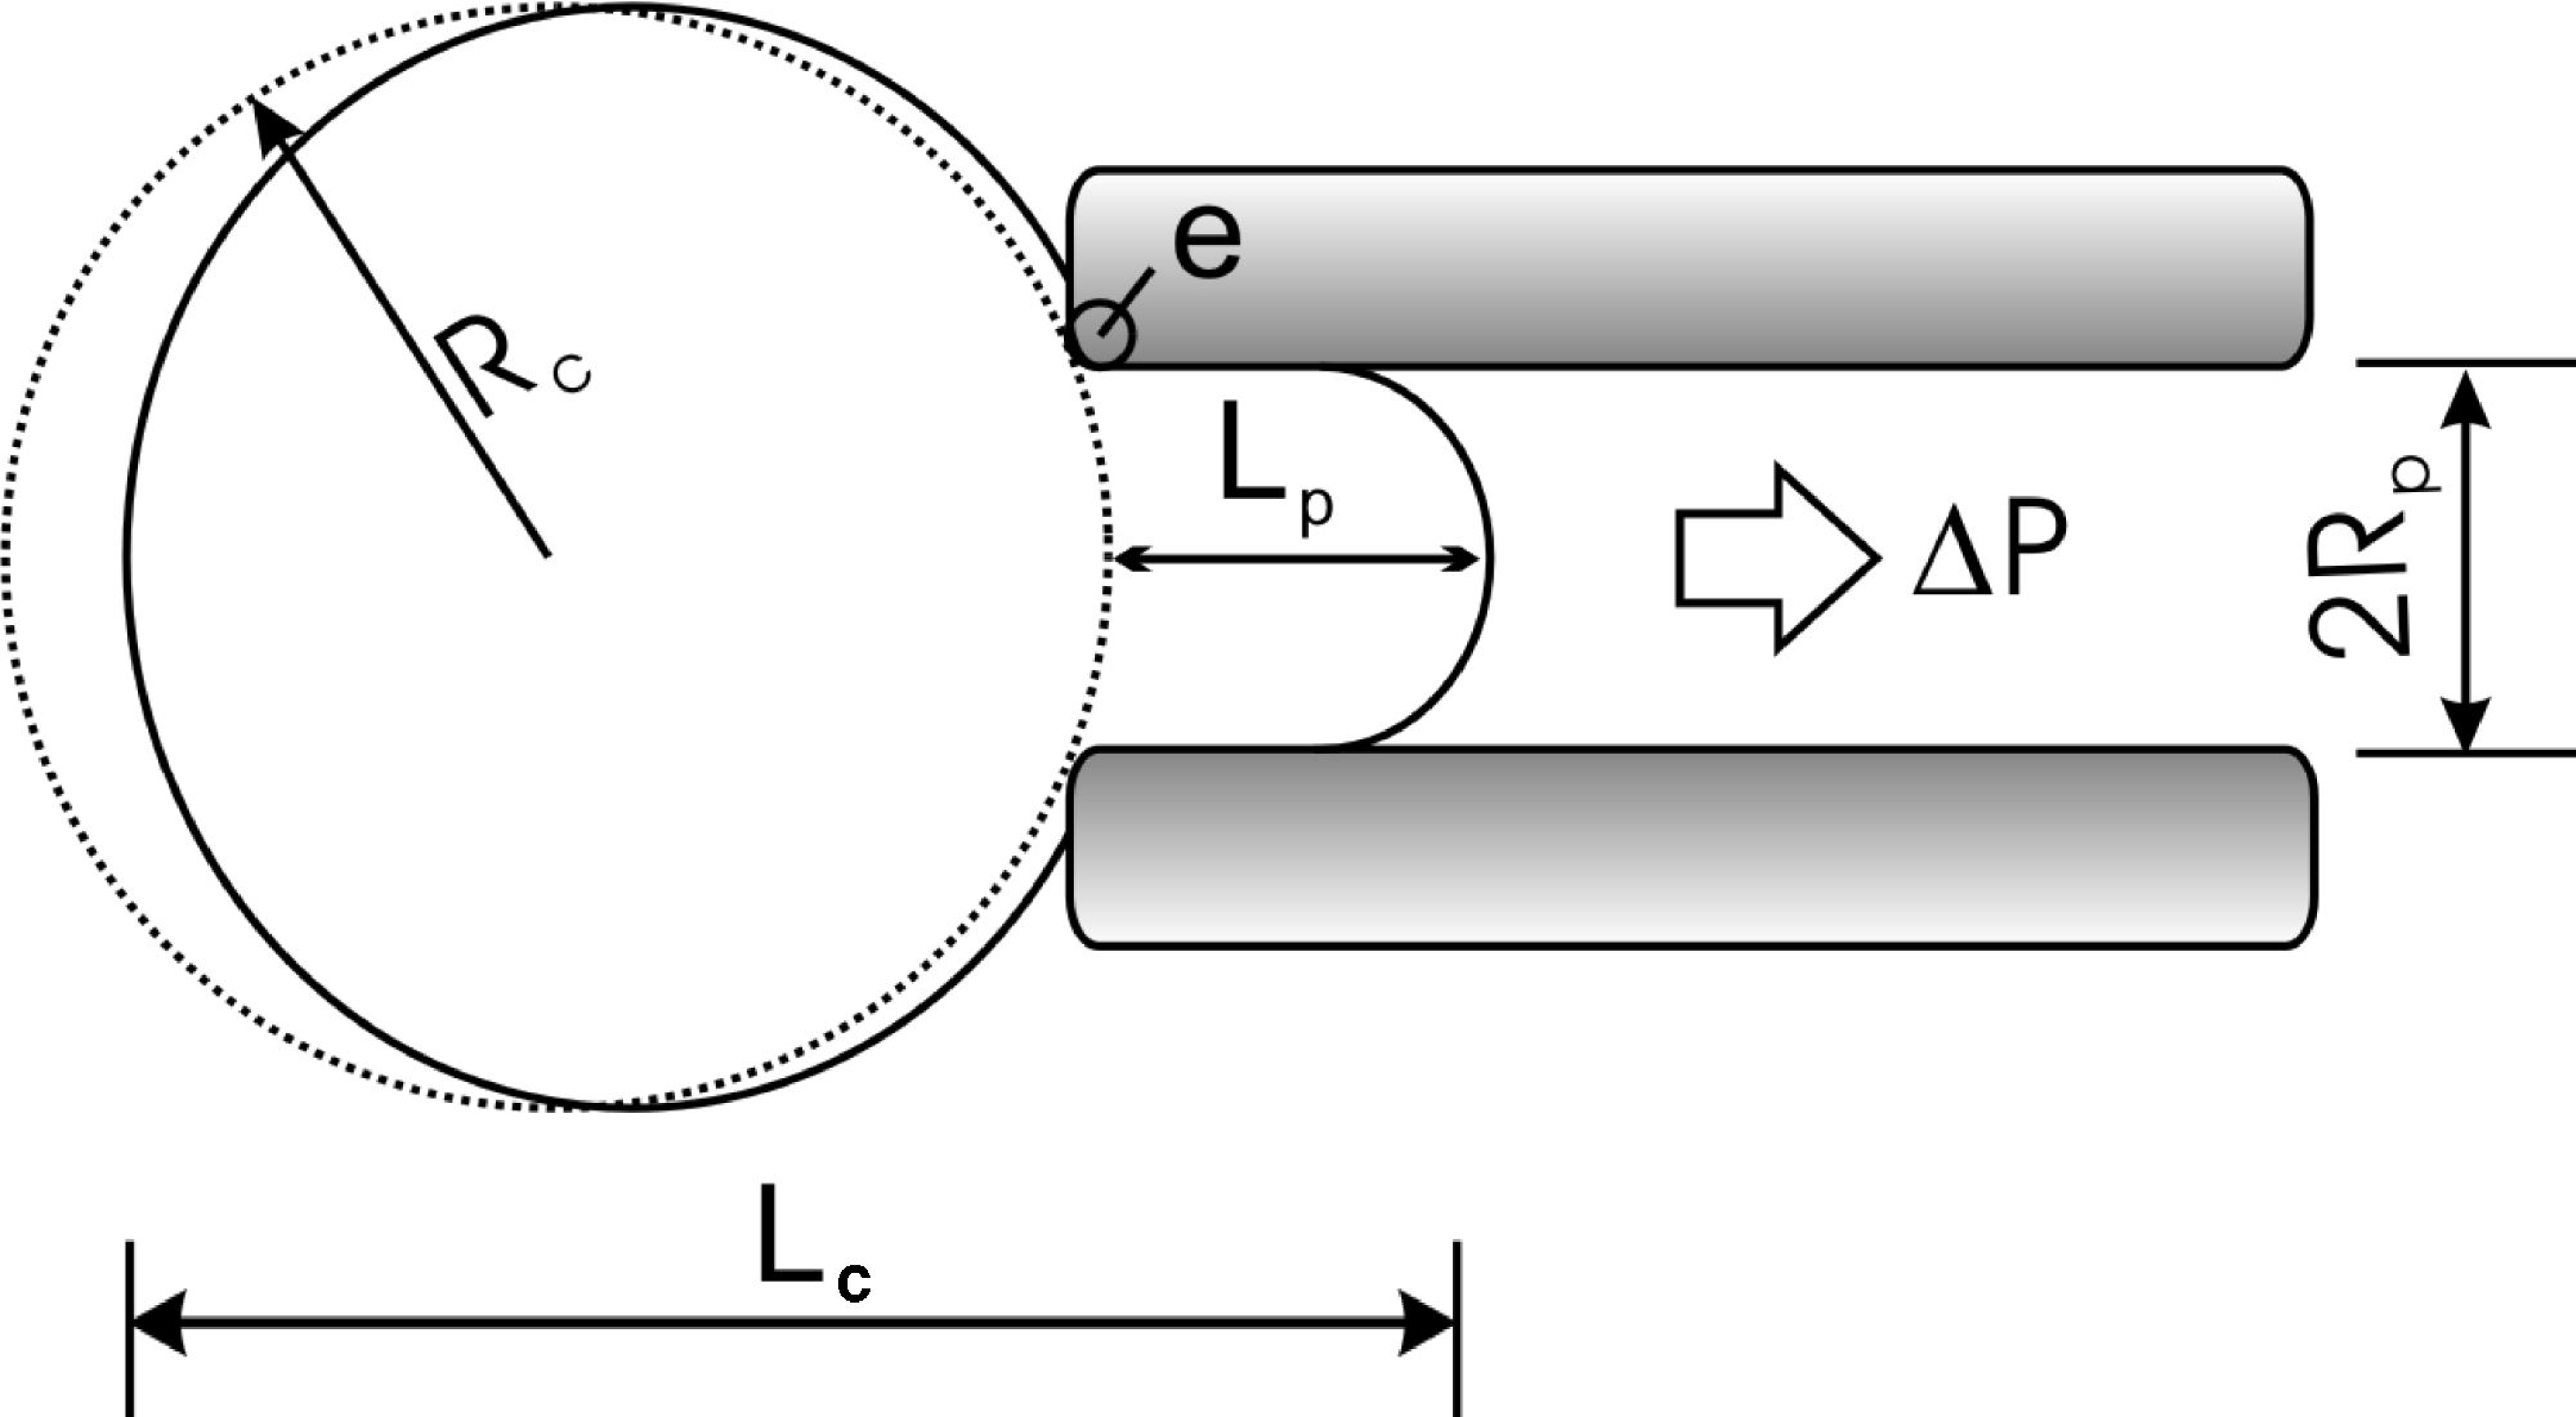
\includegraphics[width=\textwidth]{cellexp.pdf}
  \end{column}
  \begin{column}[b]{0.48\textwidth}
  \begin{itemize}
  \item 1964年, Rand和Burton首次应用微吸管测得人体红细胞膜的弹性模量.
  \item Evans和Hochmuth对细胞在微吸管实验中的变形恢复过程进行了研究.
  \end{itemize}
  \end{column}
\end{columns}
}
\subsection{细胞力学模型简介}
\frame{\frametitle{经典细胞力学模型}
\begin{columns}
  \begin{column}[b]{0.4\textwidth}
\begin{center}
 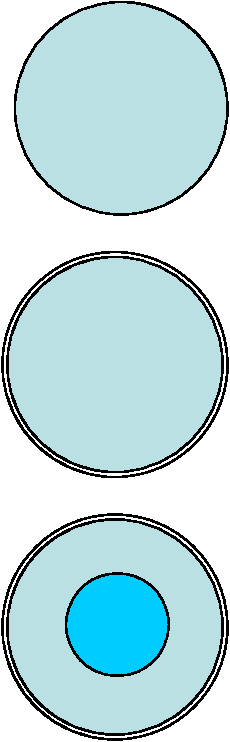
\includegraphics[width=0.3\textwidth]{model.pdf}
\end{center}
  \end{column}
  \begin{column}[b]{0.6\textwidth}
 \begin{itemize}
  \item 固体模型:细胞假设成均匀的且不含明显皮层的不可压缩弹性或者粘弹性固体.
  \item 液体模型:将细胞内部看成均匀同一的牛顿粘性流体, 细胞皮层具有张力.
  \item 复合液滴模型:在液体模型的基础上用一个封装的液滴来表示细胞核.
  \end{itemize}
  \end{column}
\end{columns}

}



\section{细胞吸入微管道的模拟}

\subsection{细胞的DPD模型}
\frame{\frametitle{FENE模型}
耗散粒子动力学模拟DNA等生物高分子流
动时, 一般采用珠簧链模型, 两个珠子之间
的弹簧力表达式为
\begin{columns}
  \begin{column}[b]{0.5\textwidth}
\begin{center}
 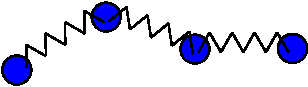
\includegraphics[width=0.6\textwidth]{FENE.pdf}
\end{center}
  \end{column}

  \begin{column}[b]{0.5\textwidth}
\[
\mathbf{F}_{ij}^S = \frac{H\mathbf{r}_ij}{1-(r_{ij}/r_{\max})^2}
\]
  \end{column}

\end{columns}
}

\frame{\frametitle{细胞的构造}
细胞膜的构造是通过FENE模型中的弹簧力将DPD粒子串联成球

  \begin{columns}
  \begin{column}[b]{0.33\textwidth}
\begin{center}
 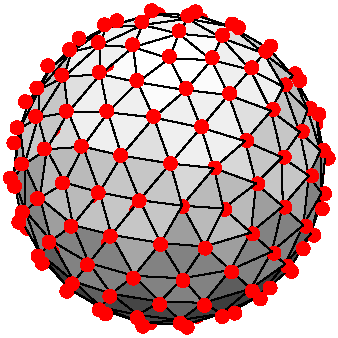
\includegraphics[width=0.8\textwidth]{p162.pdf}

$N = 162$
\end{center}
  \end{column}
  \begin{column}[b]{0.33\textwidth}
\begin{center}
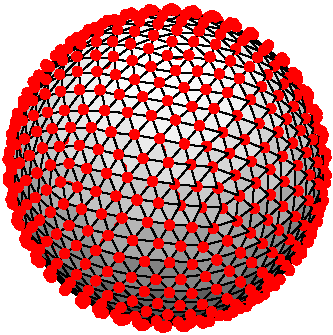
\includegraphics[width=0.8\textwidth]{p642.pdf}

$N=642$
\end{center}
  \end{column}
  \begin{column}[b]{0.33\textwidth}
\begin{center}
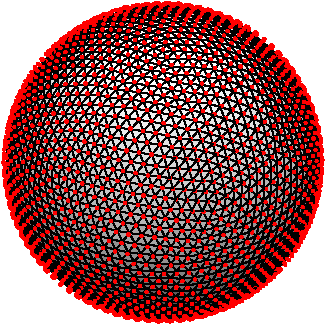
\includegraphics[width=0.8\textwidth]{p2562.pdf}

$N=2562$
\end{center}
  \end{column}
\end{columns}
}
\frame{\frametitle{模拟示意图}
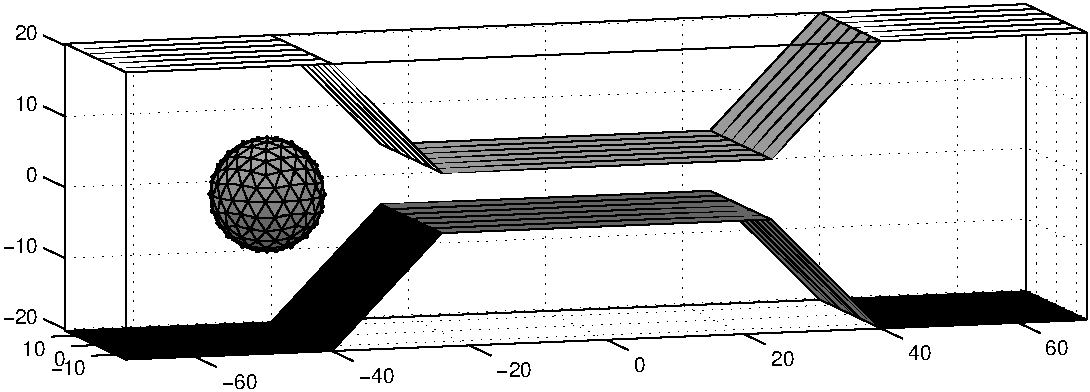
\includegraphics[width=\textwidth]{config.pdf}
}

\subsection{结果}
\frame{\frametitle{结果}
\begin{center}
  \animategraphics[width=1\textwidth, autoplay, loop]{5}{./animate/Cell/}{1}{109}
\end{center}
}

\frame{\frametitle{细胞构型}
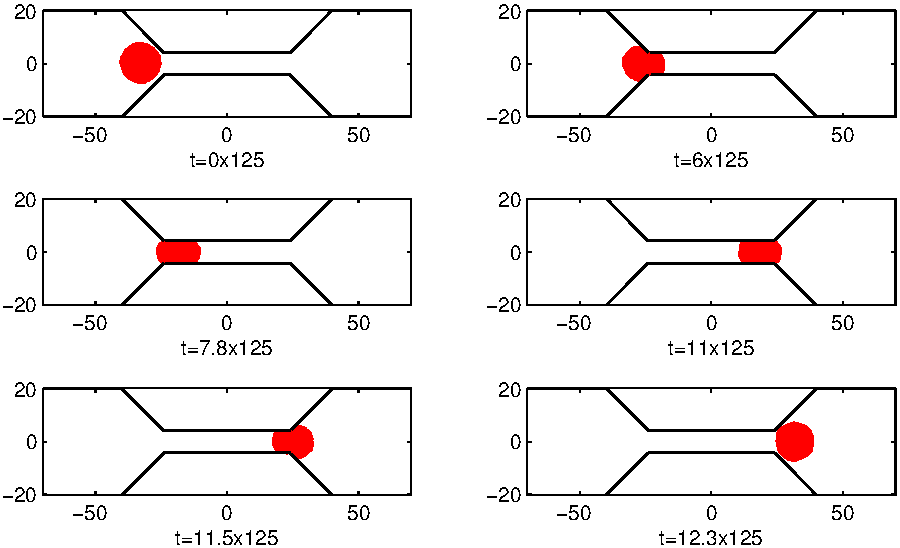
\includegraphics[width=1\textwidth]{cell.pdf}
}

\frame{\frametitle{位移与速度}
 \begin{columns}
  \begin{column}[b]{0.5\textwidth}
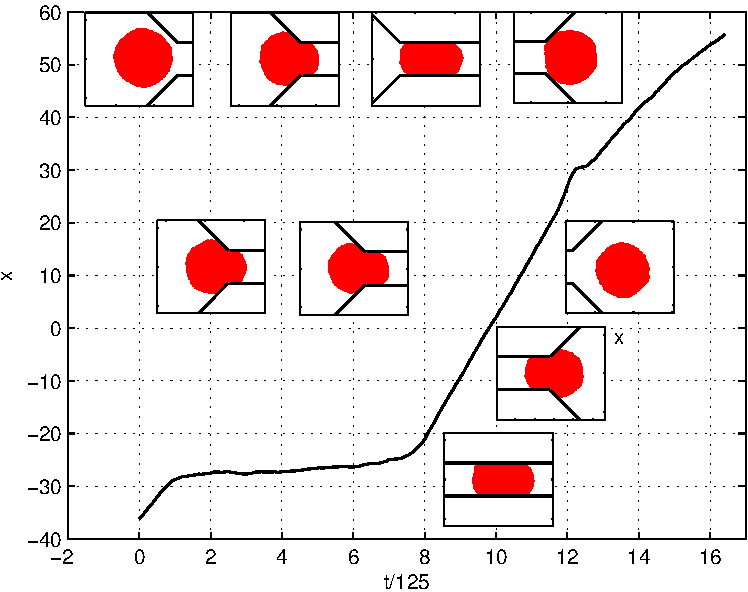
\includegraphics[width=1\textwidth]{x.pdf}
  \end{column}
  \begin{column}[b]{0.5\textwidth}
\begin{center}
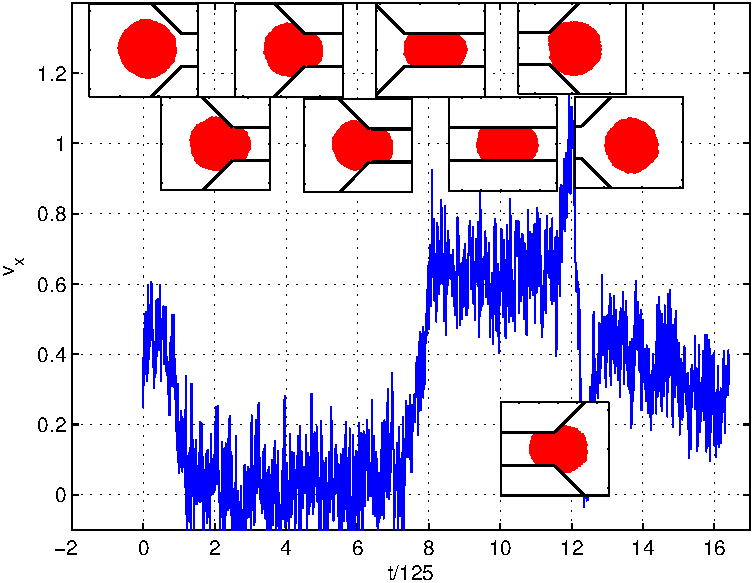
\includegraphics[width=1\textwidth]{cellLenght.pdf}
\end{center}
  \end{column}
\end{columns}
}

\frame{\frametitle{构型与实验对比}
 \begin{columns}
  \begin{column}[c]{0.5\textwidth}
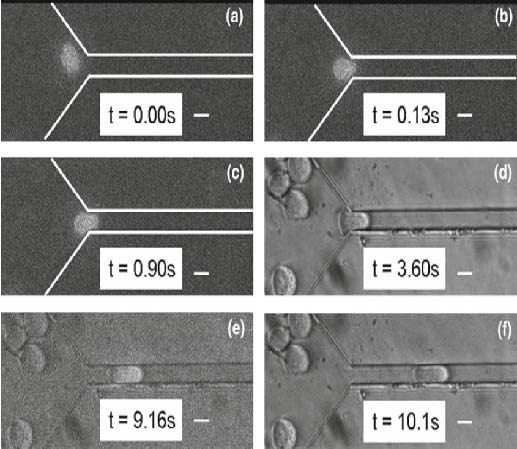
\includegraphics[width=\textwidth]{cell.jpg}
  \end{column}
  \begin{column}[c]{0.5\textwidth}
\begin{center}
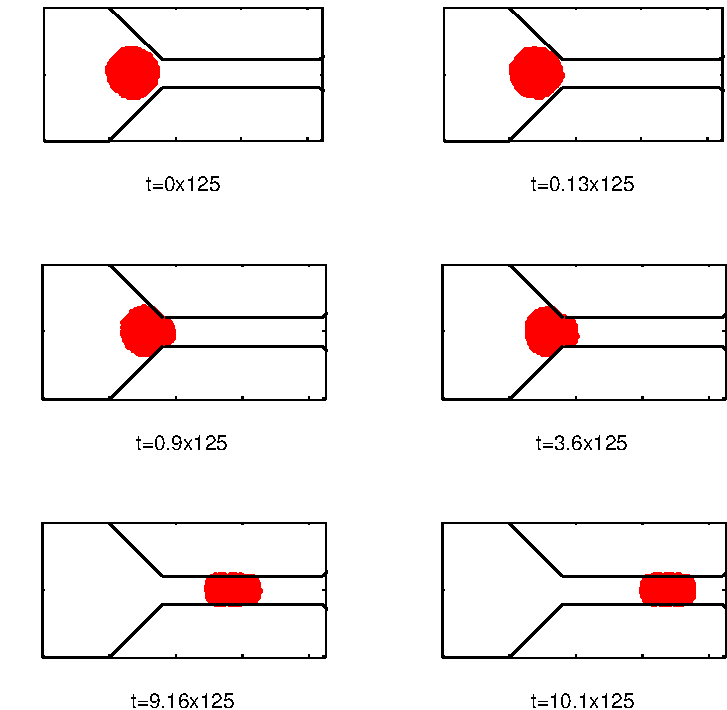
\includegraphics[width=0.98\textwidth]{cellconfig.pdf}
\end{center}
  \end{column}
\end{columns}
}

\frame{\frametitle{速度与实验对比}
 \begin{columns}
  \begin{column}[b]{0.46\textwidth}
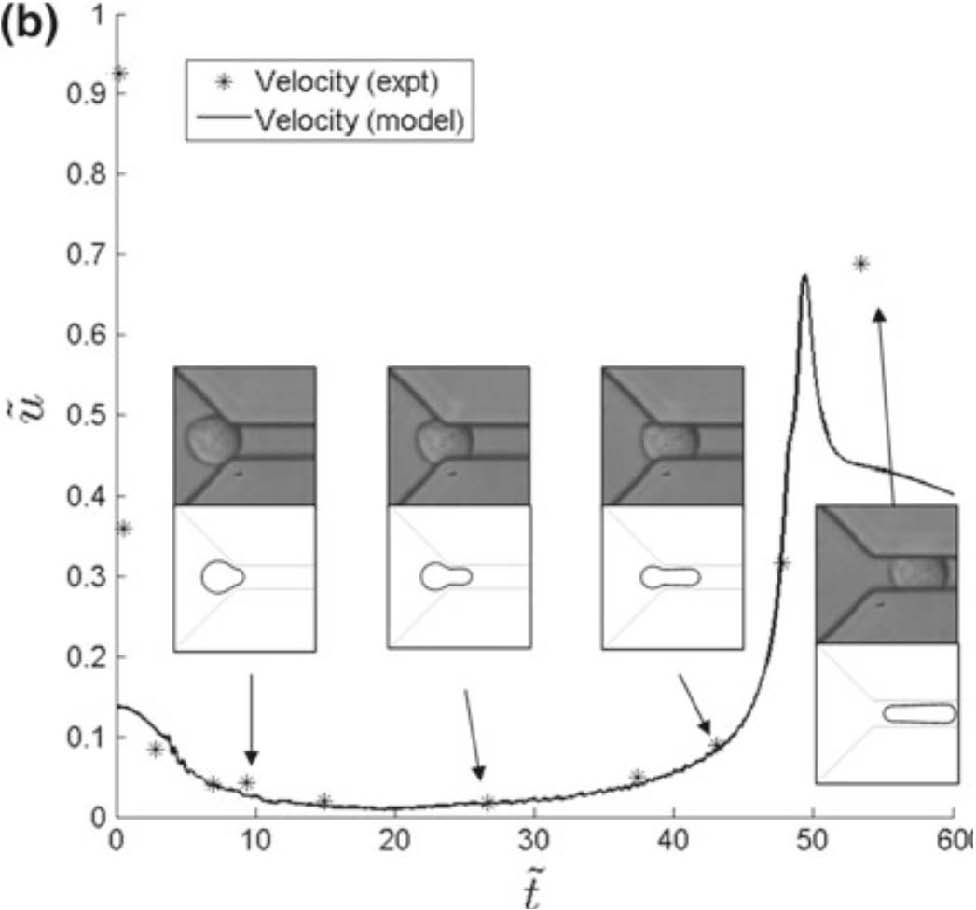
\includegraphics[width=1\textwidth]{vx.jpg}
  \end{column}
  \begin{column}[b]{0.54\textwidth}
\begin{center}
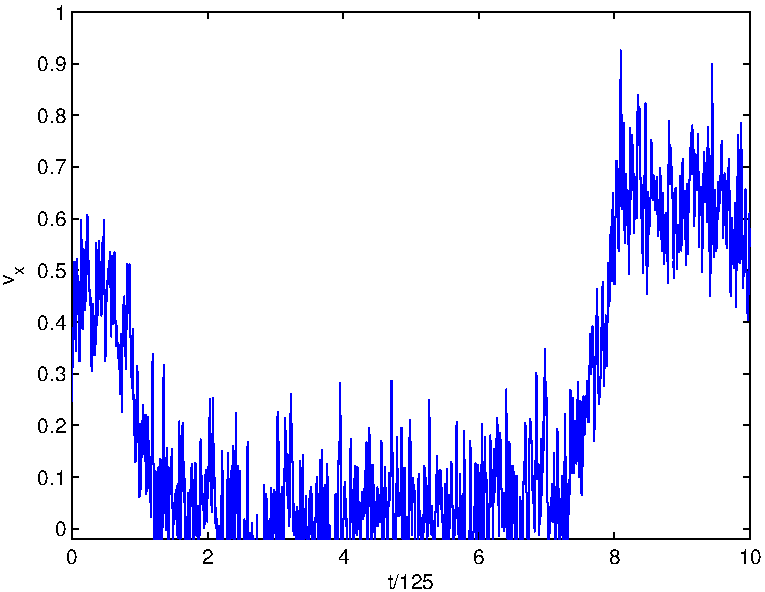
\includegraphics[width=1\textwidth]{vx.pdf}
\end{center}
  \end{column}
\end{columns}
}

\section{结论}
\frame{\frametitle{结论}
\begin{itemize}
\item 应用DPD方法及FENE珠簧链模型对细胞在微缩通道中的运动作了初步地模拟和尝试.模拟所得结果与实验基本吻合.
\item 本文的模型和模拟对于细胞的大变形和小变形都可以较好的模拟.
\item 细胞在开始进入微缩通道时减速, 拉长自身, 当细胞绝大部进入微缩结构后, 迅速加速直至细胞完全进入微缩通道; 细胞在微缩通道中的运动速度几乎不变. 当细胞从微缩结构的出口离开时, 又逐渐恢复了球形.  数值模拟所得到的细胞变形, 吸入及释放复原的形态与实验结果吻合.

\end{itemize}
}


%\section<presentation>*{参考文献}

\frame{
  \transdissolve
  \frametitle<presentation>{参考文献}

  \beamertemplatebookbibitems
  \begin{thebibliography}{10}

    \bibitem{TeX}
    Hoogerbrugge P J, Koelman J. Europhys Lett, 1992, 19: 155~160

\bibitem{TeX}
    Groot R D. J Chem Phys, 1997, 107(11): 4423~4435

\bibitem{TeX}
Espanol P, Warren P. Europhys Lett, 1995, 30(4): 191~196

    \bibitem{TeX}
    Fan X, Phan-Thien N, Yong N T, Wu X, Xu D. Phys Fluids, 2003,
15(1): 11~21

  \end{thebibliography}
}

\frame{
  \transdissolve
  \frametitle<presentation>{参考文献}

  \beamertemplatebookbibitems
  \begin{thebibliography}{10}
\bibitem{TeX}
    Rand R.P., Burton A.C. Biophysical Journal, 1964, 4:115-135

\bibitem{TeX}
Espanol P, Warren P. Europhys Lett, 1995, 30(4): 191~196

\bibitem{TeX}
C.T. Lim,, E.H. Zhou, S.T. Quek,2004,Journal of Biomechanics
39 (2006) 195–216
\bibitem{TeX}
Fong Yew Leong, Qingsen Li, Chwee Teck Lim, Keng-Hwee
Chiam. Biomech Model Mechanobiol, 2011, 10(5): 755-766

  \end{thebibliography}
}


%%%%%%%%%%%%%%%%%%%%%%%%%%%%%%%%%%%%%%%%%%%%%%%%%%%%%%%%%%%%%%%%%%%%%%%%%%
%%
%% ������һ����ʾThank you!!!�����Ķ���
%%

\newcount\opaqueness
\plainframe{
  \itshape
  \Large
    \begin{centering}
      \Huge Thank You!!!\par
    \end{centering}
} 

\end{document}
